%%%
%%% PCL Manual
%%% By Ian Johnson
%%%

\documentclass[11pt,a4paper,openright]{report}
\includeonly{%
  chapters/introduction/introduction,
  chapters/background/background,
  chapters/compiler/compiler,
  chapters/run-time/run-time
}



%%% Some commonly used packages (make sure your LaTeX installation
%%% contains these packages, if not ask your senior to help installing
%%% the packages)

\usepackage[bookmarks,%
            a4paper,%
            breaklinks,%
            backref=false,%
            dvips,ps2pdf,%
            pdfhighlight=/I,%
            pdffitwindow=true,%
            pdfstartview=Fit,%
            pdfcenterwindow=true,%
            linkbordercolor={1 0 1},%
            %colorlinks,%
            pdftitle=PCL Manual,%
            pdfauthor=Ian Johnson]%
            {hyperref}


\usepackage{cite}

\usepackage{listings}

\usepackage{amsmath}

\usepackage{natbib}
\usepackage{booktabs}
\usepackage{graphicx}
\graphicspath{{expt/}}

\usepackage{setspace}

\usepackage{times}
\usepackage[varg]{txfonts}


%%% Macro definitions for Commonly used symbols
\newcommand{\ReleaseVersion}{1.0.0}

\begin{document}
\title{\huge{Pipeline Creation Language (PCL)}\\
\LARGE{Users' Manual}\\
\normalsize{Version: \ReleaseVersion}}
\author{Ian Johnson}
\date{\today}

\maketitle

\tolerance=5000
\onehalfspacing

\begin{abstract}
PCL was developed as part of the MosesCore project sponsored by the European Commission's Seveth Framework Programme (Grant Number 288487) \url{http://www.statmt.org/mosescore/}. For more information on the Seventh Framework Programme please see \url{http://cordis.europa.eu/fp7/home_en.html}.
\end{abstract}

\pagenumbering{roman}

\tableofcontents
\listoffigures
\listoftables

\cleardoublepage
\setcounter{page}{1}
\pagenumbering{arabic}

\chapter{Introduction}

\chapter{Background}

\chapter{PCLc}

\section{Syntax}
\begin{figure}[!h]
  \centering
    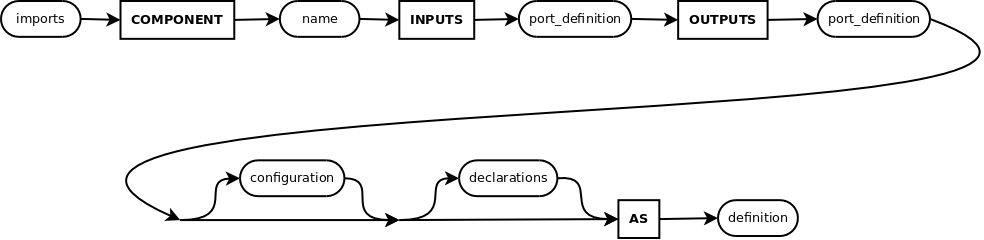
\includegraphics[width=1.0\textwidth]{chapters/compiler/diagrams/pcl-top-level}
  \caption{PCL file syntax.}
  \label{fig:pcl-top-level}
\end{figure}

\subsection{Imports}
\begin{figure}[!h]
  \centering
    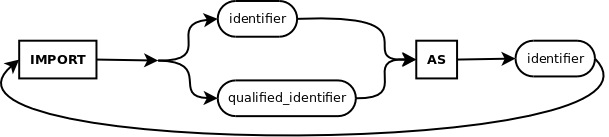
\includegraphics[width=1.0\textwidth]{chapters/compiler/diagrams/pcl-imports}
  \caption{Importing PCL files.}
  \label{fig:pcl-imports}
\end{figure}

\subsection{Port Definitions}
\begin{figure}[!h]
  \centering
    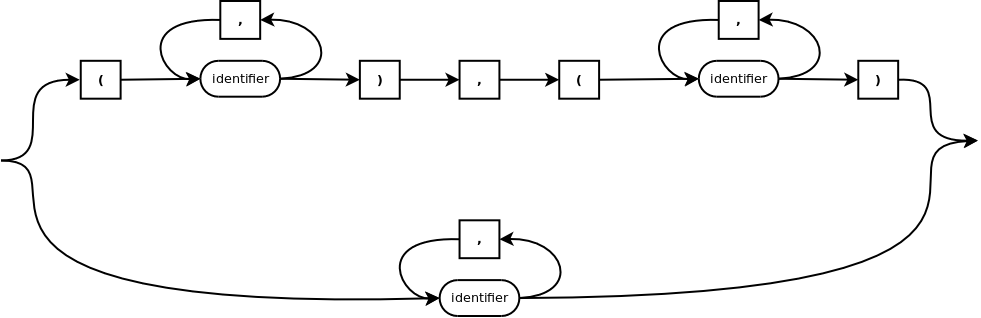
\includegraphics[width=1.0\textwidth]{chapters/compiler/diagrams/pcl-port-defs}
  \caption{Component Port Definition.}
  \label{fig:pcl-port-defs}
\end{figure}

\subsection{Configuration}
\begin{figure}[!h]
  \centering
    \includegraphics[width=1.0\textwidth]{chapters/compiler/diagrams/pcl-config}
  \caption{Component Configuraton.}
  \label{fig:pcl-config}
\end{figure}

\subsection{Declarations}

\subsection{Definition}

\chapter{PCL Runtime}


\bibliographystyle{plain}{}
\bibliography{pcl-manual}

\end{document}
